\chapter{Obesity associated genetic signatures and pathway signatures}
\label{cha:obesity_associated_genetic_signature_and_pathway_signatures}

In this chapter, the underlying biological mechanism of the obesity associated signatures from Creighton's data were investigated.
In doing so, Gatza's pathway genetic signatures were utilised to determine which biological pathways the obesity associated genetic signatures were most similar to.
First, the direction of Gatza's pathway associated genetic signatures were resolved; then the pathway associated metagenes were compared with the obesity associated metagenes; and lastly linear models were constructed based on the pathway metagenes and sample \gls{bmi}/\gls{bmi} status to predict the obesity associated metagenes.

\section{Pathway associated genetic signatures from \citet{Gatza2010a} study}
\label{sec:pathway_associated_genetic_signatures_from_gatza2010a_study}

Pathway associated genetic signatures from the \citet{Gatza2010a} study were examined for their consistency with the reported results.
In the \citet{Gatza2010a} study, their data comprised of samples from different data sets from other studies, \gls{mas}-normalised and the metagene scores were ranked with probit.
However, the analyses so far have used \gls{rma}-normalisation method and ranked based on the number of samples present in the data.
To decide which normalisation or ranking methods were suitable for the analysis, the different methods were compared in Gatza's data (see \cref{app:b}).
Results shown in \cref{app:b} clarified that there was no significant difference in the ranking methods used.
The same went for the normalisation methods, as long as the normalisation methods used to get the transformation matrix and the data in which the transformation matrix was applied to were the same.
For example, transformation matrix was taken from \gls{rma}-normalised data and then applied to \gls{rma}-normalised data set.
From these results, Gatza's data set was batch corrected first (\cref{sub:batch_correction}), then normalised with \gls{rma} method and the scores were ranked based on the number of samples in the data set.

Before Gatza's pathway metagenes were compared with the obesity associated metagenes, the direction of Gatza's pathway metagenes were checked to make sure the metagenes were in the correct direction (\cref{sub:metagene_direction}).
Each pathway metagenes was generated from Gatza's data set and the direction of the metagene was checked with the expression of the representative  pathway gene (\cref{tab:metagene_direction}).
The correlation of all the pathway metagenes with one another were plotted as a heatmap in \cref{fig:gatza_meta_dir}.
% The pathway metagenes showed a few distinct groups of pathways: a group that showed high correlation with E2F1, \gls{pi3k}, Myc, \gls{bcat} and Ras pathways; a group with \gls{ifna}, \gls{ifny} and \gls{tnfa} pathways;
The most prominent group had five pathways (E2F1, \gls{pi3k}, Myc, \gls{bcat} and Ras) that clustered at the top right hand corner of the heatmap.
% TODO: add additional info about why these pathways clustered together?
Other groups included \gls{ifna}/\gls{ifny}/\gls{tnfa} pathways, \gls{er}/\gls{pr}/p53 pathway and p63/\gls{her2} pathways.
In addition to these highly correlated groups, \gls{stat3}/\gls{tgfb}/Src/\gls{egfr}/Akt pathways showed little correlation with one another.
Comparing these groups with the results presented by \citet{Gatza2010a} (see \cref{app:b}), the identified groups approximately resembled the groups identified in their study, which confirmed that the directions of Gatza's pathway metagenes were similar to those used in the \citet{Gatza2010a} study.

\begin{figure}[htpb]
	\centering
	\includegraphics[page=15,width=0.7\linewidth]{results2/gatza_meta_trans}
	\caption{Gatza metagene direction}
	\label{fig:gatza_meta_dir}
\end{figure}

To see whether the directionality of Gatza's pathway metagenes were being transferred across to other data sets properly, pathway metagenes were generated with the transformation matrices and the groupings of the metagenes were examined.
Creighton's, FM's and Cris' data were \gls{rma}-normalised and transformation matrices of the pathway genetic signatures were applied to the data.
The metagenes were plotted in a heatmap (shown in \cref{app:b}).
These heatmaps showed similar groupings  as seen in \cref{fig:gatza_meta_dir}, which proved that the directions of the pathway metagenes were independent of the data sets.


% In order to investigate what the underlying biological mechanism of the obesity associated genetic signatures was, Gatza's pathway associated genetic signatures were used to create linear models to predict the obesity associated metagene scores.
% Before linear models were created, Gatza's pathway metagenes were checked for their directionality to ensure that the pathway metagenes were acting as reported by \citet{Gatza2010a} (see \cref{sub:metagene_direction}).

\section{Pathway associated metagenes and obesity associated metagenes}
\label{sec:pathway_associated_metagenes_and_obesity_associated_metagenes}

Results from previous section confirmed that the pathway metagenes from the \citet{Gatza2010a} study were in the correct directions.




then the pathway associated metagenes were compared with the obesity associated metagenes







\section{Prediction of obesity associated metagene with pathway associate metagene}
\label{sec:prediction_of_obesity_associated_metagene_with_pathway_associate_metagene}

and lastly linear models were constructed based on the pathway metagenes and sample \gls{bmi}/\gls{bmi} status to predict the obesity associated metagenes.





